%%%%%%%%%%%%%%%%%%%%%%%%%%%%%%%%%%%%%%%%%%%%%%%%%%%%%%%%%%%%%%%%%%%
%                                                                 %
%   FFREAD User Guide and Reference manual                        %
%                                                                 %
%   Front Material                                                %
%                                                                 %
%   Editor: Jamie Shiers/ CN-ASD                                  %
%   Last Mod.: 14 Feb 1994 14:40 jds                              %
%                                                                 %
%%%%%%%%%%%%%%%%%%%%%%%%%%%%%%%%%%%%%%%%%%%%%%%%%%%%%%%%%%%%%%%%%%%

%%%%%%%%%%%%%%%%%%%%%%%%%%%%%%%%%%%%%%%%%%%%%%%%%%%%%%%%%%%%%%%%%%%%
%    Tile page                                                     %
%%%%%%%%%%%%%%%%%%%%%%%%%%%%%%%%%%%%%%%%%%%%%%%%%%%%%%%%%%%%%%%%%%%%
\def\Ptitle#1{\special{ps: /Printstring (#1) def}
                       \epsfbox{cnastit.eps}}
 
\begin{titlepage}
\vspace*{-23mm}
\mbox{\epsfig{file=cern15.eps,height=30mm}}
\hfill
\raise8mm\hbox{\Large\bf CERN Program Library Long Writeups I302}
\hfill\mbox{}
\begin{center}
  \mbox{}\\[6mm]
  \mbox{\Ptitle{FFREAD}}\\[2cm]
  {\LARGE Format Free Input Processing}\\[2cm]
  {\LARGE Version 3.13}\\[3cm]
  {\Large Application Software and Databases Group}\\[6mm]
  {\Large Computing and Networks Division}\\[2cm]
\end{center}
\vfill
\begin{center}\Large CERN Geneva, Switzerland\end{center}
\end{titlepage}

\Filename{H1Preface}

\Filename{H2Copyright}

%%%%%%%%%%%%%%%%%%%%%%%%%%%%%%%%%%%%%%%%%%%%%%%%%%%%%%%%%%%%%%%%%%%%
%    Copyright  page                                               %
%%%%%%%%%%%%%%%%%%%%%%%%%%%%%%%%%%%%%%%%%%%%%%%%%%%%%%%%%%%%%%%%%%%%
\thispagestyle{empty}
\framebox[\textwidth][t]{\hfill\begin{minipage}{0.96\textwidth}%
\vspace*{3mm}
\begin{center}Copyright Notice\end{center}

\parskip.6\baselineskip
CERN Program Library entry \textbf{Q123}

\textbf{FFREAD -- Format Free Input Processing}

\copyright{} Copyright CERN, Geneva 1993
 
Copyright and any other appropriate legal protection of these
computer programs and associated documentation reserved in all
countries of the world.
 
These programs or documentation may not be reproduced by any
method without prior written consent of the Director-General
of CERN or his delegate.
 
Permission for the usage of any programs described herein is
granted apriori to those scientific institutes associated with
the CERN experimental program or with whom CERN has concluded
a scientific collaboration agreement.
 
Requests for information should be addressed to:
\vspace*{-.5\baselineskip}
\begin{center}
\tt\begin{tabular}{l}
CERN Program Library Office              \\
CERN-CN Division                         \\
CH-1211 Geneva 23                        \\
Switzerland                              \\
Tel.      +41 22 767 4951                \\
Fax.      +41 22 767 7155                \\
Bitnet:   CERNLIB@CERNVM                 \\
DECnet:   VXCERN::CERNLIB (node 22.190)  \\
Internet: CERNLIB@CERNVM.CERN.CH
\end{tabular}
\end{center}
\vspace*{2mm}
\end{minipage}\hfill}%end of minipage in framebox
\vspace{6mm}
 
{\bf Trademark notice: All trademarks appearing in this guide are acknowledged as such.}
\vfill

\begin{tabular}{l@{\quad}l@{\quad}>{\small\tt}l}
{\em Contact Person\/}:        & CERN Program Library& (CERNLIB\atsign CERN.CH)\\[1mm]
{\em Technical Realization\/}: & Michel Goossens /CN & (Michel.GOOSSENS\atsign CERN.CH)\\[2cm]
\textem{Edition -- February 1994}
\end{tabular}
\newpage

\Filename{H2Prelimininary-remarks}

%%%%%%%%%%%%%%%%%%%%%%%%%%%%%%%%%%%%%%%%%%%%%%%%%%%%%%%%%%%%%%%%%%%%
%    Introductory material                                         %
%%%%%%%%%%%%%%%%%%%%%%%%%%%%%%%%%%%%%%%%%%%%%%%%%%%%%%%%%%%%%%%%%%%%
\pagenumbering{roman}
\setcounter{page}{1}

\section*{Preliminary remarks}

\begin{center}
\fbox{\parbox{12cm}{Throughout this manual, commands to be \textbf{entered}
are {\tt\Ucom{underlined}}}}
\end{center}

\index{underlining}
\index{user input}

This document has been produced using \LaTeX~\cite{bib-LATEX}
with the \Lit{cernman} style option, developed at CERN. 
A compressed PostScript file \Lit{ffread.ps.gz}, 
containing a complete printable version
of this manual, can be obtained from any CERN machine
by anonymous ftp as follows
(commands to be typed by the user are underlined)\footnote{%
If your site does not carry the gnu \Lit{gzip} utility you can get the
uncompressed file by dropping the \Lit{.gz} suffix from the
\Ucom{get} command, and also skipping the \Ucom{binary}
specification below.}:

\begin{XMP}
    \Ucom{ftp asis01.cern.ch}
    Trying 128.141.201.136...
    Connected to asis01.cern.ch.
    220 asis01 FTP server (Version 6.10 ...) ready.
    Name (asis01:username): \Ucom{anonymous}
    Password: \Ucom{your\_{}mailaddress}
    230 Guest login ok, access restrictions apply.
    ftp> \Ucom{cd cernlib/doc/ps.dir}
    ftp> \Ucom{binary}
    ftp> \Ucom{get ffread.ps.gz}    ! one page per physical page
    ftp> \Ucom{quit}
\end{XMP}


%%%%%%%%%%%%%%%%%%%%%%%%%%%%%%%%%%%%%%%%%%%%%%%%%%%%%%%%%%%%%%%%%%%%
%    Tables of contents ...                                        %
%%%%%%%%%%%%%%%%%%%%%%%%%%%%%%%%%%%%%%%%%%%%%%%%%%%%%%%%%%%%%%%%%%%%
\newpage
\tableofcontents
